\documentclass[UTF8,11pt]{ctexart}

\usepackage[margin=0.75in]{geometry}
\usepackage{amsmath}
\usepackage{array}
\usepackage{booktabs}
\usepackage{float}
\usepackage{graphicx}
\usepackage{hyperref}
\usepackage{xcolor}
\usepackage{url}

\setCJKmainfont{Noto Sans CJK SC}
\hypersetup{
  colorlinks=true,
  linkcolor=blue!55!black,
  urlcolor=blue!55!black,
  citecolor=blue!55!black
}

\title{Yichao 逐 z 明场到荧光预测性能报告}
\author{OrganoidAgent}
\date{2026 年 5 月 20 日}

\begin{document}
\maketitle

\section*{摘要}

本文档记录已经完成的 Yichao 逐 z 明场到荧光（B2F, brightfield-to-fluorescence）实验。任务是：从类器官的明场裁剪图预测对应的、经过背景/伪信号抑制后的荧光目标。模型只用 Data-Yichao-1 到 Data-Yichao-10 训练、验证和内部测试；Data-Yichao-11 是完全独立的外部测试集，没有参与训练、验证或 checkpoint 选择。

最容易理解的外部测试指标是荧光区域 F1。在 Data-Yichao-11 上，逐 z 模型的最佳 support F1 为 \(0.454\)，固定阈值 F1 为 \(0.418\)。Data-Yichao-11 的阳性 support 像素比例约为 \(0.071\)，所以这个 F1 明显不是随机猜测。模型预测的总荧光量是真实总荧光量的 \(1.135\times\)，也就是整体高估约 \(13.5\%\)。因此，当前模型已经学到了真实的明场-荧光关联，但还不是像素级完美重建。

\section*{任务定义}

这里的目标来自荧光图，不是明场图。在当前 Yichao 数据约定中，\(c1\) 是明场，\(c0\) 是荧光。对每个分割出来的类器官实例：
\[
B_i = \text{明场裁剪图}, \quad
F_i = \text{原始荧光裁剪图}, \quad
Y_i = \text{清理后的连续荧光目标}.
\]
模型预测一个单通道连续目标：
\[
\hat{Y}_i = G_\theta(B_i, M_i, D_i),
\]
其中 \(M_i\) 是类器官分割 mask，\(D_i\) 是由分割 mask 得到的距离图辅助通道。二值荧光 support mask \(S_i\) 是从 \(Y_i\) 里推导出来，用于 support loss 和指标计算。它不是明场的二值 mask。

\begin{figure}[H]
  \centering
  \fbox{\begin{minipage}{0.92\textwidth}
  \[
  \text{明场 }(c1) + \text{类器官 mask} + \text{距离图}
  \;\xrightarrow{\text{hybrid U-Net}}\;
  \text{来自 }c0\text{ 的单通道清理荧光目标}
  \]
  \[
  \text{连续目标学习强度；support loss 学习稀疏阳性荧光区域}
  \]
  \end{minipage}}
  \caption{B2F 任务流程。输入是明场形态和分割得到的辅助通道，输出是荧光图衍生出来的连续目标。}
\end{figure}

\section*{数据}

主实验把每一个原始 z 平面都当作一个独立样本，不做 z 投影。这样可以保留深度信息，便于之后做时间/深度建模。报告中也加入了最大明场/最大荧光投影实验作为对照，因为它能提供一个单图像投影版本的性能参考。

\begin{table}[H]
  \centering
  \caption{数据和划分数量。Data-Yichao-11 只作为外部测试集。}
  \resizebox{\textwidth}{!}{\begin{tabular}{@{}llr@{}}
\toprule
数据阶段 & 定义 & 数量 \\
\midrule
逐 z 原始图像 & Data 1--11 的明场/荧光图像记录 & 79,405 \\
逐 z 实例记录 & 分割得到的类器官实例记录 & 354,797 \\
边缘填充实例 & 接触裁剪边界或图像边界的实例 & 132,997 \\
逐 z 可用目标 & Data 1--10 过滤后用于构建目标的行数 & 214,311 \\
训练集 & Data 1--10 训练划分 & 139,935 \\
验证集 & Data 1--10 验证划分 & 62,814 \\
内部测试集 & Data 1--10 内部测试划分 & 11,562 \\
外部测试集 & Data-Yichao-11，完全不参与训练 & 7,489 \\
\midrule
最大投影可用目标 & Data 1--10 投影后的训练目标 & 9,775 \\
最大投影外部测试 & Data-Yichao-11 投影后的测试目标 & 420 \\
\bottomrule
\end{tabular}
}
\end{table}

\begin{figure}[H]
  \centering
  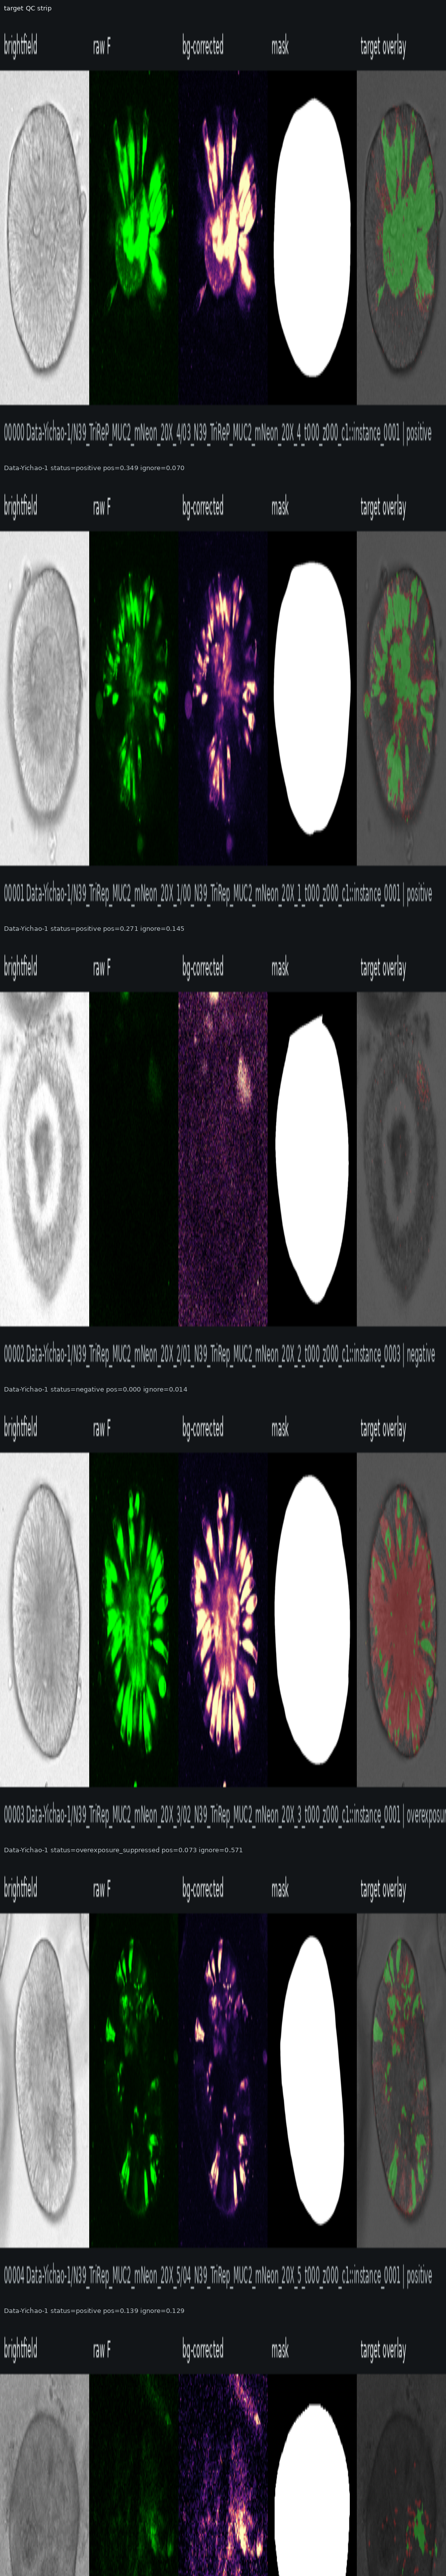
\includegraphics[height=0.82\textheight]{figures/fig2_training_target_qc_gallery.png}
  \caption{训练目标 QC 图的代表性截取。图中展示明场、原始荧光、清理后的连续荧光目标，以及用于定义学习目标的 support 表示。}
\end{figure}

\section*{模型和损失函数}

模型是 hybrid U-Net 风格的 image-to-image 网络，输入大小为 256 像素，输出为单通道。输入通道数为 3：明场、类器官 mask、距离图。训练使用 CUDA，batch size 为 12，base channels 为 32，dropout 为 0.05，学习率为 \(1.5\times10^{-4}\)，weight decay 为 \(2\times10^{-4}\)，总共训练 500 个 epoch。每个 epoch 用 balanced sampler 抽取 20,000 个训练样本。

目标是归一化并裁剪到 \([0,1]\) 的单通道背景抑制荧光信号。损失函数同时包含连续回归和 support 学习：
\[
\mathcal{L}
= \mathcal{L}_{1,w}
+0.25\,\mathcal{L}_{\mathrm{MSE},w}
+0.5\,\mathcal{L}_{\mathrm{softDice}}
+\mathcal{L}_{\mathrm{focal}}
+0.2\,\mathcal{L}_{\mathrm{total}}
+0.08\,\mathcal{L}_{\mathrm{background}}.
\]
这个设计避免让模型只学习一个严格的黑白二值 mask。连续目标保留荧光强度信息，soft-Dice 和 focal support loss 则帮助模型关注稀疏的阳性荧光区域，避免被大量背景像素淹没。

\section*{指标解释}

\begin{table}[H]
  \centering
  \caption{主要指标解释。F1 是最容易理解的区域检测指标；总强度比和总强度 log 相关用于解释表达量尺度。}
  \resizebox{\textwidth}{!}{\begin{tabular}{@{}lll@{}}
\toprule
指标 & 衡量内容 & 实际解释 \\
\midrule
最佳 F1 & 在不同阈值下寻找最佳荧光区域 F1 & 最直观的荧光区域检测准确度 \\
0.2 阈值 F1 & 固定阈值 0.2 下的荧光区域 F1 & 一个固定操作点下的准确度 \\
总强度比 & 预测荧光总量 / 真实荧光总量 & 接近 1 说明总表达量校准较好 \\
总强度 log 相关 & 每个实例总荧光强度的 log 相关 & 是否能正确排序强/弱表达类器官 \\
Pearson & 像素级连续强度相关 & 精细空间强度是否一致 \\
阳性 Pearson & 只在真实阳性荧光像素内计算相关 & 阳性区域内部强度预测质量 \\
\bottomrule
\end{tabular}
}
\end{table}

\section*{性能}

\begin{table}[H]
  \centering
  \caption{验证集、内部测试集和外部测试集主要性能。最大投影外部测试作为对照。}
  \resizebox{\textwidth}{!}{\begin{tabular}{@{}lrrrrrrr@{}}
\toprule
评估集合 & 行数 & Pearson & 阳性 Pearson & 最佳 F1 & 0.2 阈值 F1 & 总强度比 & 总强度 log 相关 \\
\midrule
验证集，最佳 epoch 210 & 62,814 & 0.449 & 0.230 & 0.477 & 0.447 & 1.016 & 0.587 \\
验证集，epoch 500 & 62,814 & 0.442 & 0.233 & 0.476 & 0.432 & 0.976 & 0.539 \\
内部测试，Data 1--10 & 11,562 & 0.189 & 0.180 & 0.225 & 0.129 & 0.466 & 0.358 \\
外部测试，Data-Yichao-11 & 7,489 & 0.333 & 0.041 & 0.454 & 0.418 & 1.135 & 0.580 \\
外部测试，Data-Yichao-11 最大投影 & 420 & 0.288 & -0.020 & 0.482 & 0.429 & 0.828 & 0.355 \\
\bottomrule
\end{tabular}
}
\end{table}

逐 z 模型的最佳验证 checkpoint 在 epoch 210，support 最佳 F1 为 \(0.477\)，固定阈值 F1 为 \(0.447\)，总强度比为 \(1.016\)。最终 epoch 500 的验证表现接近，但完整 pipeline 使用最后一个 epoch 对 Data-Yichao-11 做外部评估。

最重要的是 Data-Yichao-11 外部测试。逐 z 模型在这个完全未参与训练的数据上达到 support 最佳 F1 \(=0.454\)，固定阈值 F1 \(=0.418\)，总强度比 \(=1.135\)。这说明模型能大致找到荧光区域，并能估计总荧光量级，但还不能称为像素级完美重建。

内部测试集 Data 1--10 的 F1 比外部 Data-Yichao-11 低，说明内部 test split 包含更困难或分布不同的样本。因此解释模型时不能只看一个数值，而需要同时看内部测试、外部测试和可视化结果。

\begin{figure}[H]
  \centering
  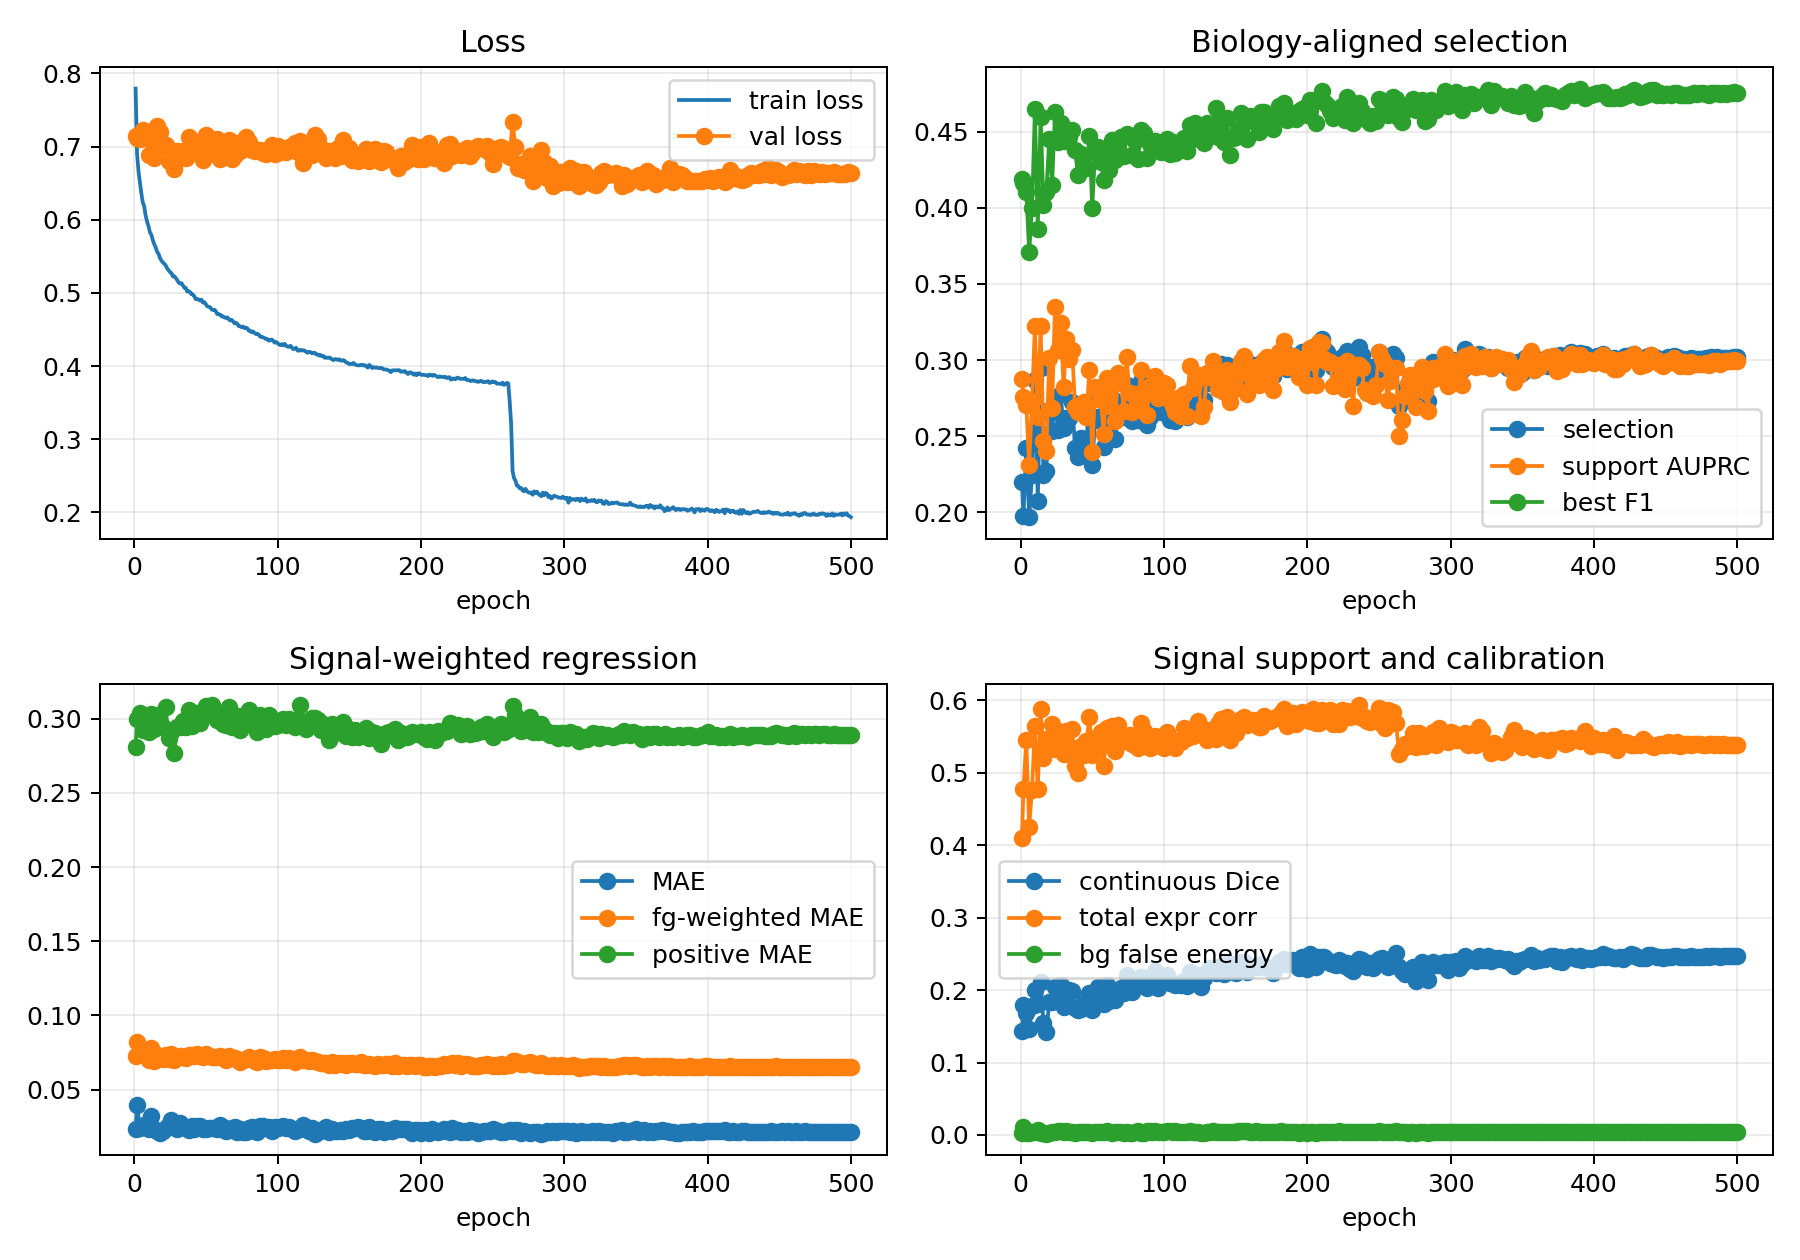
\includegraphics[width=\textwidth]{figures/fig1_per_z_training_metrics.png}
  \caption{逐 z 模型 500 epoch 训练和验证曲线。}
\end{figure}

\section*{预测可视化}

\begin{figure}[H]
  \centering
  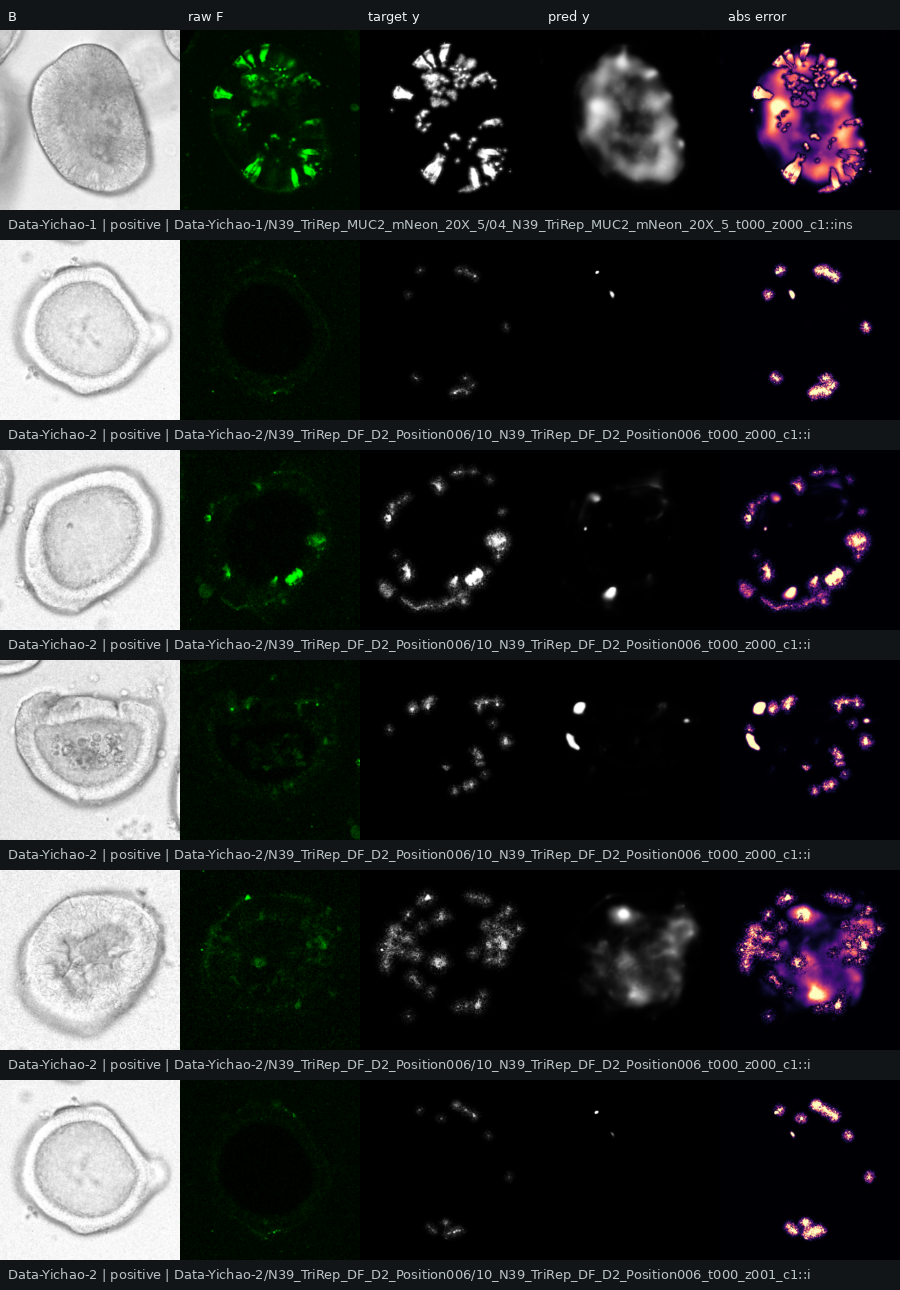
\includegraphics[height=0.82\textheight]{figures/fig3_internal_test_panel.png}
  \caption{逐 z 模型内部测试 panel，使用 Data 1--10 中的 held-out test 行。}
\end{figure}

\begin{figure}[H]
  \centering
  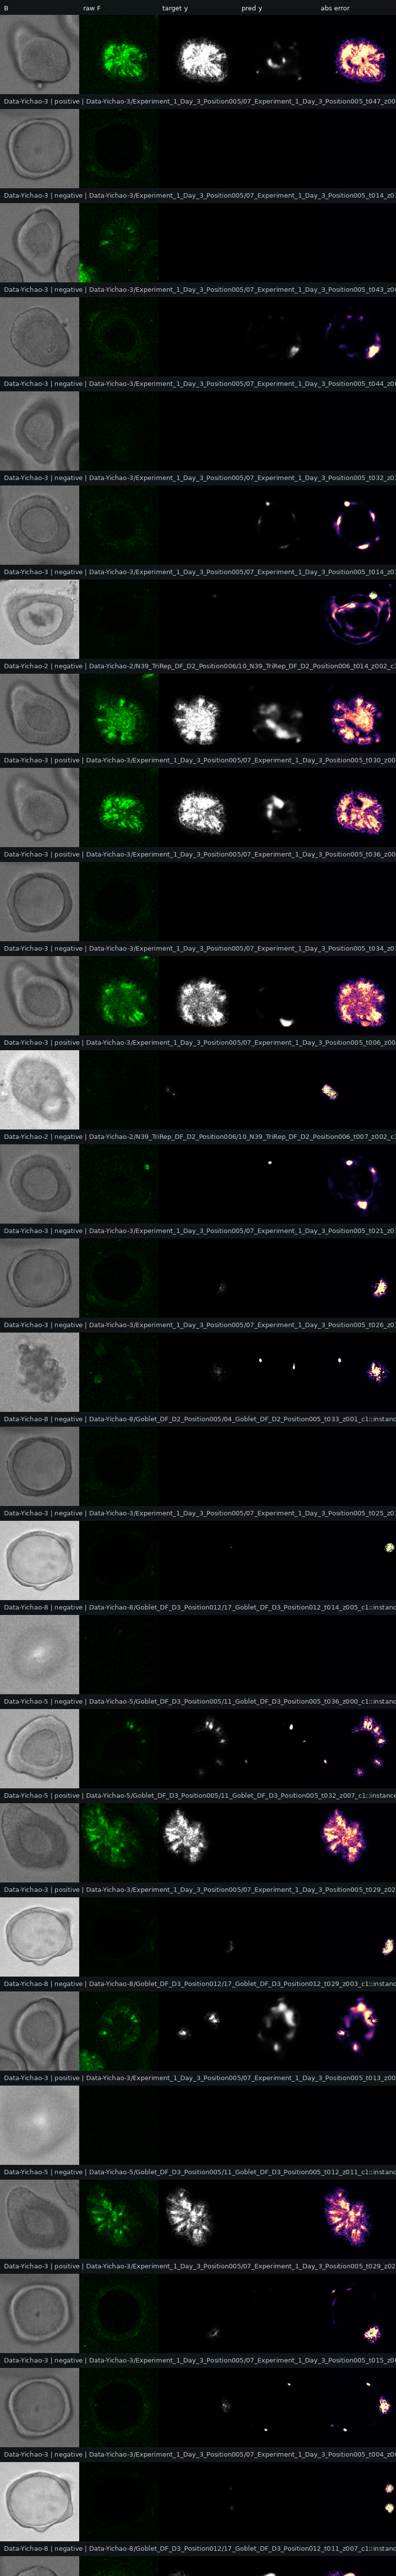
\includegraphics[height=0.82\textheight]{figures/fig4_internal_test_gallery.png}
  \caption{内部测试随机 gallery 的代表性截取。可视化检查很重要，因为区域 F1 和像素相关会反映不同类型的错误。}
\end{figure}

\begin{figure}[H]
  \centering
  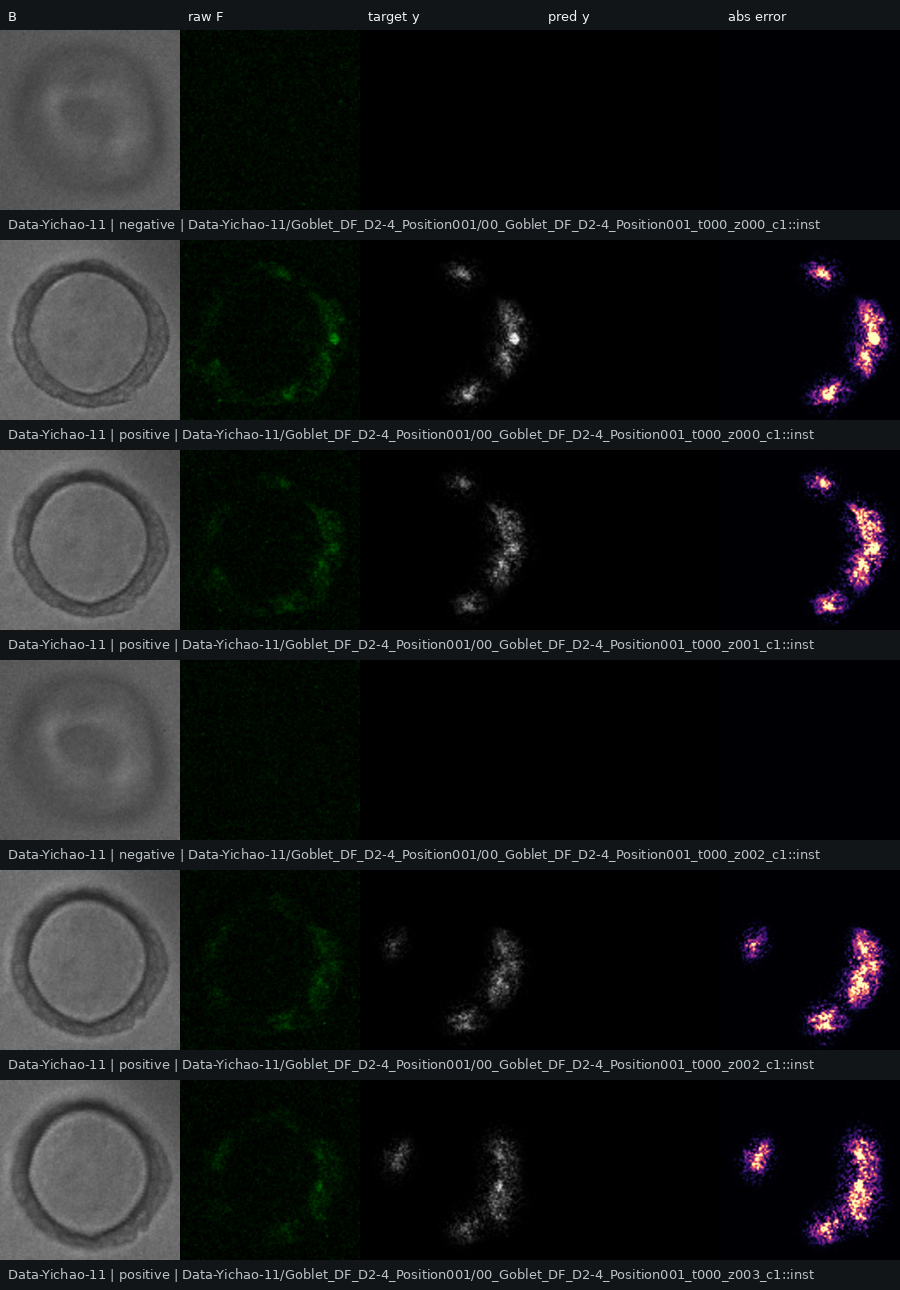
\includegraphics[height=0.82\textheight]{figures/fig5_external_data11_panel.png}
  \caption{Data-Yichao-11 外部测试预测 panel。Data-Yichao-11 从未用于训练或验证。}
\end{figure}

\begin{figure}[H]
  \centering
  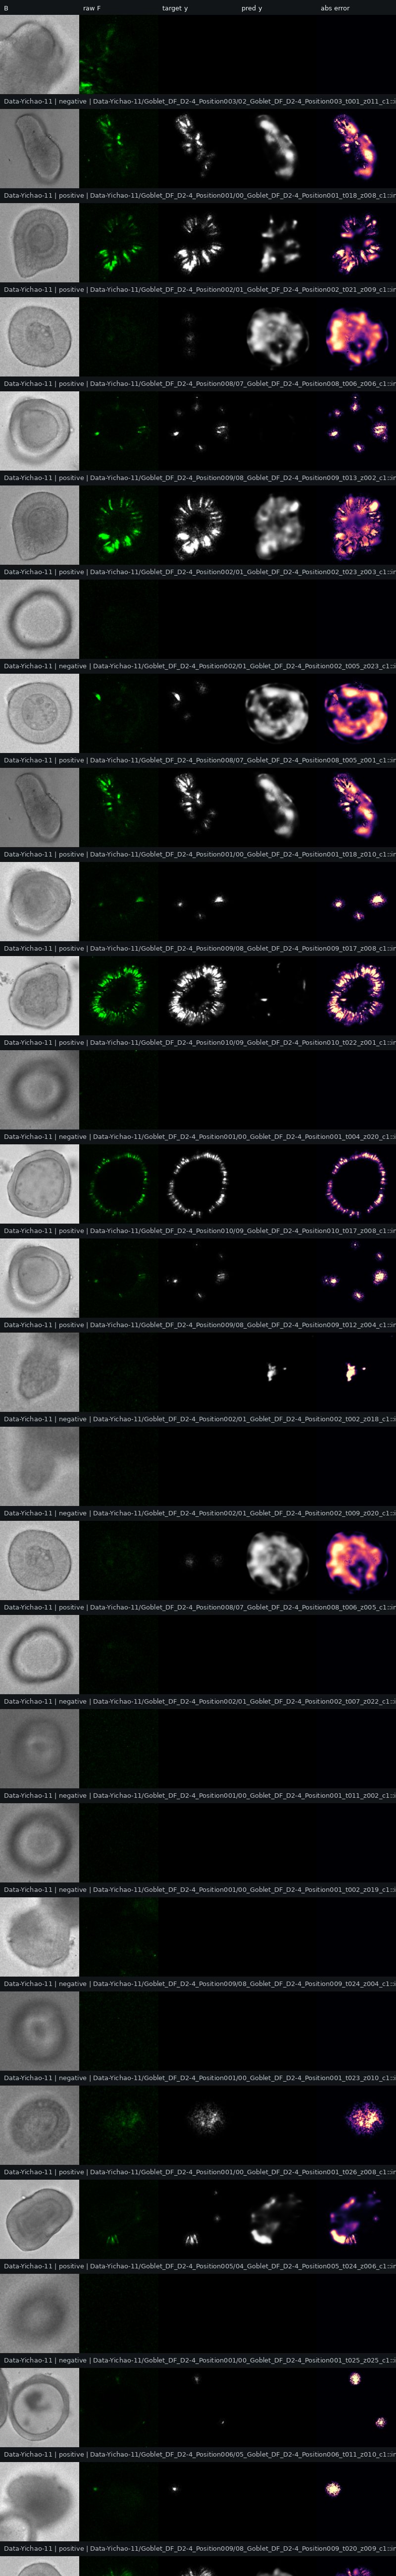
\includegraphics[height=0.82\textheight]{figures/fig6_external_data11_gallery.png}
  \caption{Data-Yichao-11 外部测试随机 gallery 的代表性截取。模型通常能在粗尺度上找到正确的荧光阳性区域，但细节强度仍不完美。}
\end{figure}

\begin{figure}[H]
  \centering
  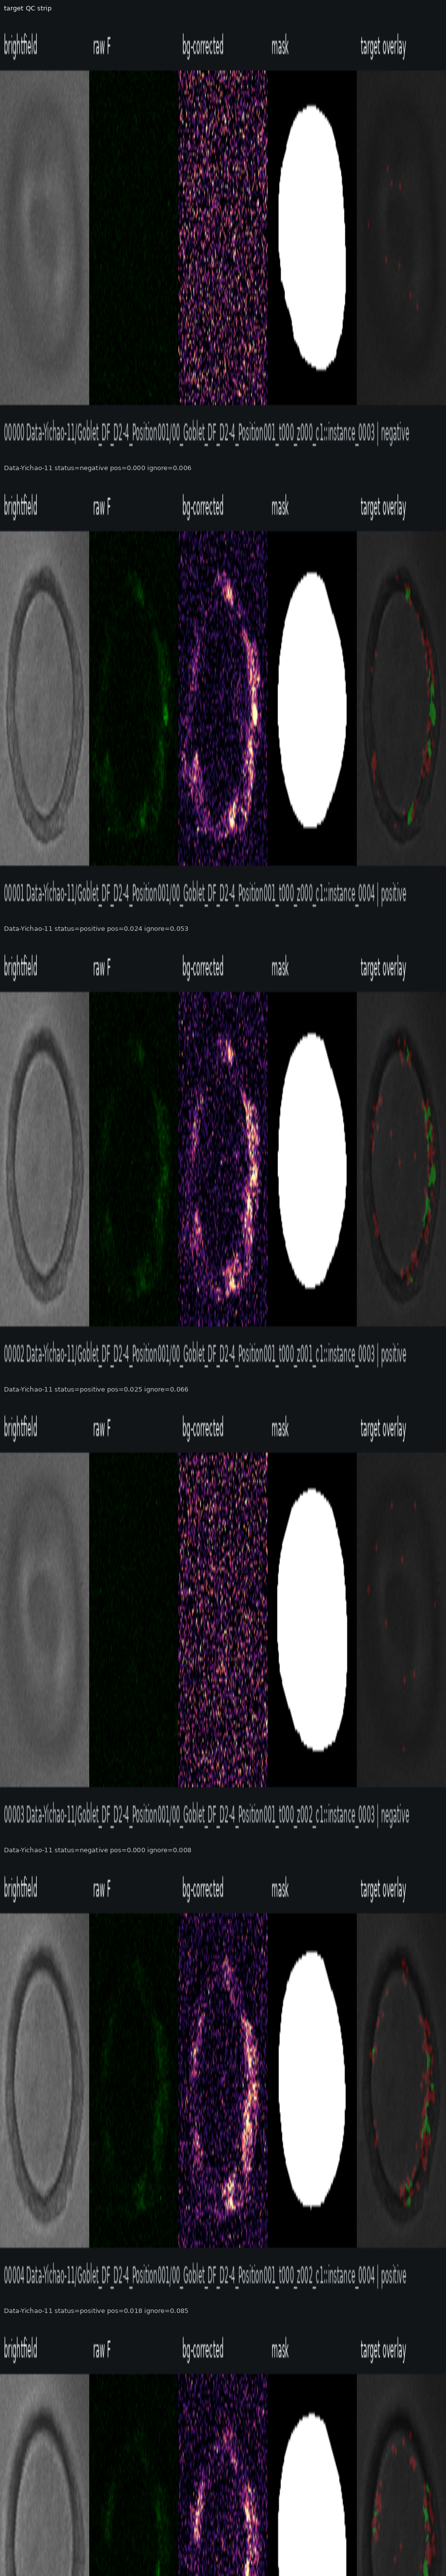
\includegraphics[height=0.82\textheight]{figures/fig7_external_data11_target_qc.png}
  \caption{Data-Yichao-11 外部测试目标 QC 图的代表性截取，展示模型评估时使用的荧光衍生目标。}
\end{figure}

\section*{与最大投影方法比较}

最大投影实验把所有 z 平面压缩成每个时间/位置一个投影实例。它的样本量更少，但单图像目标更干净。在 Data-Yichao-11 上，最大投影 support 最佳 F1 为 \(0.482\)，略高于逐 z 模型的 \(0.454\)。但是最大投影的总强度比为 \(0.828\)，逐 z 模型为 \(1.135\)；并且逐 z 模型在 Data-Yichao-11 上的总强度 log 相关更高（\(0.580\) 对 \(0.355\)）。

\begin{figure}[H]
  \centering
  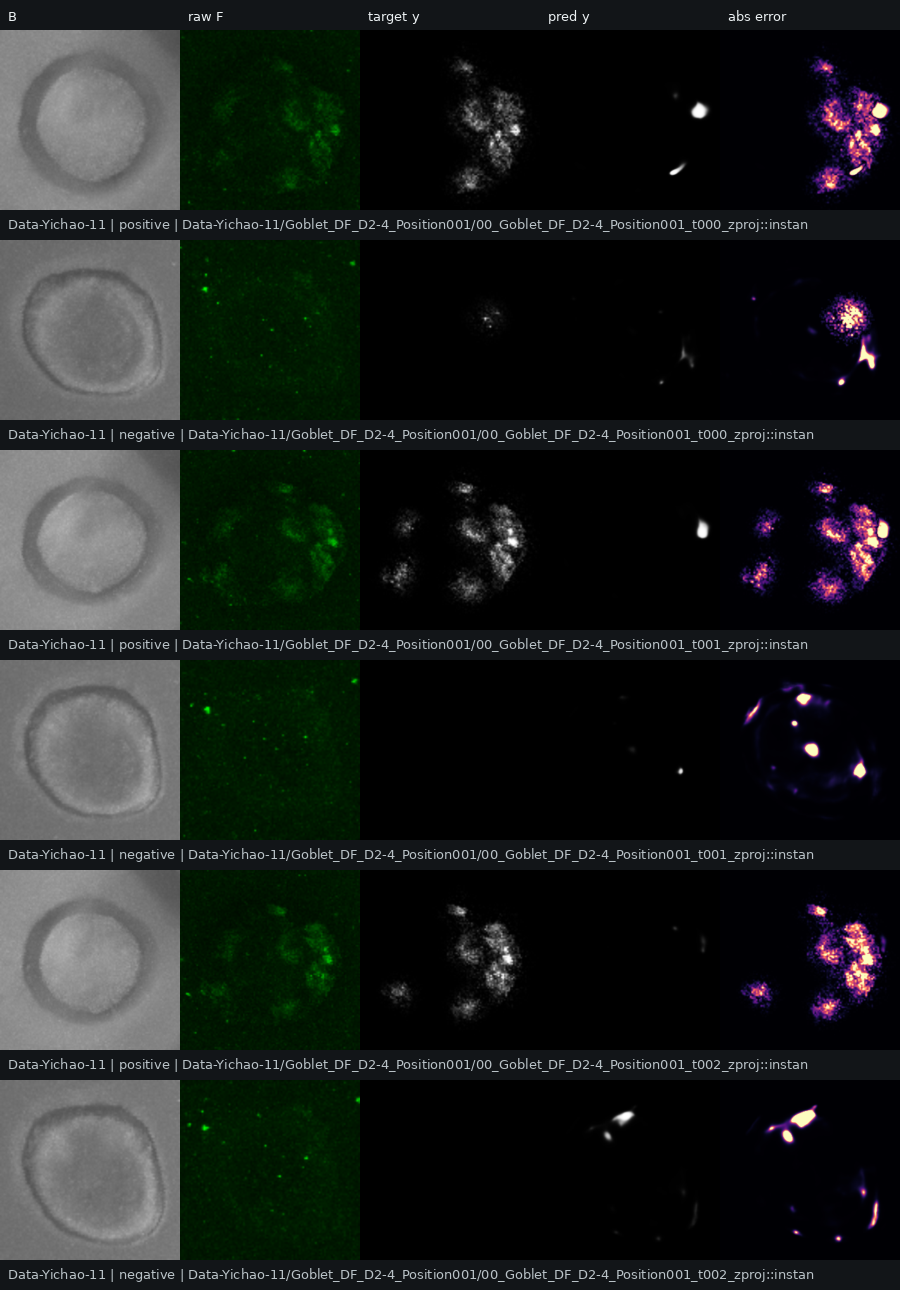
\includegraphics[height=0.82\textheight]{figures/fig8_max_projection_data11_panel.png}
  \caption{Data-Yichao-11 最大投影外部测试对照图。投影可以略微提高区域 F1，但会丢掉 z 方向结构。}
\end{figure}

\section*{结论和下一步}

当前结果是有价值的。外部测试 F1 \(=0.454\) 明显高于阳性 support 像素比例 \(0.071\)，并且总荧光量接近真实尺度。因此模型不是随机猜测，而是学到了明场形态与荧光表达之间的关系。

主要弱点不是模型完全学不到，而是阳性区域内部的细粒度强度相关仍然偏低，尤其在外部 Data-Yichao-11 上更明显。下一步应保留当前“连续目标 + support loss”的设计，同时加强校准和时间一致性。对于未来表达预测，更合理的路线是把这个 B2F 模型作为表征或辅助任务，再结合时间序列、位置、深度和表达起始点，而不是只依赖单帧同时间像素预测。

\section*{主要文件路径}

\begin{itemize}
\item 逐 z 总结：\path{/home/lachlan/ProjectsLFS/OrganoidAgent/analysis-outputs/yichao_per_z_b2f_pipeline/summary.md}
\item 逐 z 模型目录：\path{/home/lachlan/ProjectsLFS/OrganoidAgent/analysis-outputs/yichao_fluorescence_continuous/runs/per_z_1to10_hybrid_unet_v1_500}
\item Data-Yichao-11 外部指标：\path{/home/lachlan/ProjectsLFS/OrganoidAgent/analysis-outputs/yichao_external_tests/Data-Yichao-11_per_z/evaluation/Data-Yichao-11_per_z_last_epoch_external_metrics.json}
\item Markdown 参考文档：\path{/home/lachlan/ProjectsLFS/OrganoidAgent/references/Yichao/per_z_b2f_performance_report.md}
\end{itemize}

\end{document}
